\chapter{Experiment Setup And Execution}
\section{Goals}
As already mentioned this study is investigating the coverage of the parts which already can be automatically optimized by Polly, the various reasons for these parts not being even larger and the impact to the coverage and the speedup if these reasons could be eliminated.

\section{Measurement Methology}
For measuring, analysis and evaluation of the results the following definitions are introduced.
\subsection{Definition Coverage}
Let \(T_i\in\mathbb{N}\) be the execution time of all instructions within all \scops of a project and \(T\in\mathbb{N}\) the overall execution time of that project.
Then the coverage of parallelizable regions \(DynCov\in\mathbb{Q}\) is defined as:
\[DynCov := \frac{T_i}{T}\]

\subsection[Amdahl's Law]{Amdahl's Law \cite{AmdahlsLaw}}
Let \(N\in\mathbb{N}\) be the number of processors and \(DynCov\in\mathbb{Q}\) be the coverage of parallelizable regions.
Then the speedup \(S\in\mathbb{Q}\) is defined as:
\[S := \frac{N}{(1-DynCov)*N+DynCov}\]
\subsection{Reasons for SCoPs being invalid}
These are the criteria implemented by Polly for rejecting a parent of a \scop being also a \scop.
Some of these criteria are referencing to a \llvm specific value called \undefv \cite{llvmUndef}.
\begin{itemize}
    \item Parent is top level (\autoref{lst:parentIsToplevel})\\
        This is simply when the parent of a \scop is a top level region.
        Per default a top level region can not be a \scop in Polly.
    \item Unsupported terminator instruction\\
        This is occurring when a flow breaking instruction like \texttt{return}, \texttt{throw} or \texttt{goto} is called within a loop.
    \item Unreachable in exit block (\autoref{lst:unreachableExitBlock})\\
        This is appearing when \texttt{unreachable()} is called within an exit block \cite{llvmUnreachable}.
    \item Irreducible regions (\autoref{lst:irreducibleLoops})\\
        \Eg a region is interfering with another region using labels.
        So that the loop can not be changed in general.
    \item Undefined branch condition\\
        It is occurring whenever at least a part of a branch condition is based on the value \undefv.
    \item Non-integer branch condition\\
        Appears if the branch condition is neither constant nor using an integer comparison.
    \item Undefined operands in comparison\\
        Arises when the value \undefv is used in a comparison.
    \item Non-affine branch condition\\
        This is the case if the branch is not affine like it contains a function call.
    \item No base pointer\\
        Occurs if a base pointer is missing.
    \item Undefined base pointer\\
        It is raised when a base pointer holds the value \undefv.
    \item Variant base pointer (\autoref{lst:variantBasePointer})\\
        Occurs when a base pointer in a region is not invariant.
    \item Non-affine memory accesses (\autoref{lst:nonAffineMemoryAccesses})\\
        This is appearing when accessing memory in a non-affine way like using \(i^2\) as access steps.
        More precisely: Appears if the array subscript of an access is not affine.
    \item Accesses with differing sizes\\
        Arises if an array is accessed using data types of differing sizes.
    \item Uncomputable loop bounds (\autoref{lst:uncomputeableLoopBounds})\\
        Appears if Polly fails to derive an affine loop bound \eg the loop bounds could not be computed because they are depending on an input parameter.
    \item Loop without exit (\autoref{lst:loopWithoutExit})\\
        Occurs if the loop has no exit or if not all latches are part of the loop region.
    \item Function call with side effects (\autoref{lst:functionCallSideEffects})\\
        This is raised when a function is called which is not guaranteed to have no side effects or at least it is not known whether it has side effects.
    \item Complicated access semantics (volatile or atomic)\\
        Arises if memory is accessed which is not \enquote{simple}.
        This means the keywords volatile is used or an atomic variable is accessed.
    \item Base address aliasing (\autoref{lst:baseAddressAliasing})\\
        Occurs if Polly can not determine whether two pointer are accessing the same memory or -- when talking about arrays -- whether these arrays overlap.
    \item Integer to pointer conversion (\autoref{lst:integerToPointer})\\
        This occurs when a regular int is used as pointer somewhere into the memory.
    \item Stack allocations\\
        Stack allocations like using \texttt{alloca} can not be handled.
    \item Unknown instructions\\
        Arises if an instruction is used where Polly knows no definition.
    \item Contains entry block\\
        Polly is yet not able to handle regions which contain the entry of a function.
    \item Assumed to be unprofitable (\autoref{lst:assumedUnprofitable})\\
        When the region is very small or it is not likely that an optimization improves the execution it is left out.
        This means at least Polly is not able to find a profitable polyhedral optimization for the given region.
        As already mentioned in this study also these unprofitable regions are discussed.
    \item Polly does not return a reason\\
        When requesting the reason for a region not being a \scop Polly may return an empty string.
        This occurs if the Log object used internally has errors or if it does not exist at all.
\end{itemize}

\begin{comment}
    Following is copy\&pasted from pollys ScopDetectionDiagnostic.cpp

SCOP_STAT(CFG, ""),
SCOP_STAT(InvalidTerminator, "Unsupported terminator instruction"),
SCOP_STAT(UnreachableInExit, "Unreachable in exit block"),
SCOP_STAT(IrreducibleRegion, "Irreducible loops"),
SCOP_STAT(LastCFG, ""),
SCOP_STAT(AffFunc, ""),
SCOP_STAT(UndefCond, "Undefined branch condition"),
SCOP_STAT(InvalidCond, "Non-integer branch condition"),
SCOP_STAT(UndefOperand, "Undefined operands in comparison"),
SCOP_STAT(NonAffBranch, "Non-affine branch condition"),
SCOP_STAT(NoBasePtr, "No base pointer"),
SCOP_STAT(UndefBasePtr, "Undefined base pointer"),
SCOP_STAT(VariantBasePtr, "Variant base pointer"),
SCOP_STAT(NonAffineAccess, "Non-affine memory accesses"),
SCOP_STAT(DifferentElementSize, "Accesses with differing sizes"),
SCOP_STAT(LastAffFunc, ""),
SCOP_STAT(LoopBound, "Uncomputable loop bounds"),
SCOP_STAT(LoopHasNoExit, "Loop without exit"),
SCOP_STAT(FuncCall, "Function call with side effects"),
SCOP_STAT(NonSimpleMemoryAccess,
          "Compilated access semantics (volatile or atomic)"),
SCOP_STAT(Alias, "Base address aliasing"),
SCOP_STAT(Other, ""),
SCOP_STAT(IntToPtr, "Integer to pointer conversions"),
SCOP_STAT(Alloca, "Stack allocations"),
SCOP_STAT(UnknownInst, "Unknown Instructions"),
SCOP_STAT(Entry, "Contains entry block"),
SCOP_STAT(Unprofitable, "Assumed to be unprofitable"),
SCOP_STAT(LastOther, "")
\end{comment}

\section{Experiment Variables}
The experiment variables are listed in \autoref{tab:experimentVariables}.\\
The classification \(C\) describes two types of regions handled within the study.
The one is \enquote{\scop} like explained in \autoref{subsec:definitionScop}.
The other is \enquote{parent} which is the next bigger region surrounding a \scop.\\
The variables \dyncovs and \dyncovp are depending on \(TI\) because the selection of tests to run influences the regions executed and how often they are executed.
So \(TI\) has to be controlled.
This is done by using on the one hand integrated benchmarks brought by the tested programs and on the other hand using benchmarks which are accepted by the community like SPEC2006. (see \autoref{tab:subjectPrograms})\\
Also the speedups \(S_s\) and \(S_p\) are dependent because they are calculated out of \dyncovs and \dyncovp.
\begin{table}[H]
    \myfloatalign
    \small
    \begin{tabularx}{\textwidth}{Xccccc} \toprule
        \tableheadline{Name}              & \tableheadline{Abbr.} & \tableheadline{Type} & \tableheadline{Scale Type} & \tableheadline{Unit}                          & \tableheadline{Range} \\ \midrule
        Classification                    & \(C\)                 & Indep.               & Nominal                    & \makecell{\{Parent,\\\scop\}}                 & Text\\
        Test inputs                       & \(TI\)                & Con.                 & Nominal                    & \makecell{see\\\autoref{tab:subjectPrograms}} & Text\\
        \midrule
        Coverage of \scops                & \dyncovs              & Dep.                 & Ratio                      & \%                                            & \([0; 1[ \in \mathbb{Q}\)\\
        Coverage of MaxRegions            & \dyncovp              & Dep.                 & Ratio                      & \%                                            & \([0; 1[ \in \mathbb{Q}\)\\
        Theoretical speedup of \scops     & \(S_s\)               & Dep.                 & Ratio                      & \%                                            & \([0; 1[ \in \mathbb{Q}\)\\
        Theoretical speedup of MaxRegions & \(S_p\)               & Dep.                 & Ratio                      & \%                                            & \([0; 1[ \in \mathbb{Q}\)\\
        \bottomrule
    \end{tabularx}
    \caption[Experiment Variables]{
        Experiment variables (Dep.=Dependent; Indep.=Independent; Con.=Controlled).
        The term \enquote{MaxRegions} contains all regions classified as parent and the \scops which have only a parent which is a top level region.
    }
    \label{tab:experimentVariables}
\end{table}
Besides the experiment variables also the term \enquote{MaxRegions} has to be introduced.
MaxRegions contains all regions classified as parent and the \scops which have only a parent which is a top level regions.

\section{Hypotheses}
\(H_1\): The main reason for rejecting a \scop should be that its parent already is a top level region because also all \scops classified as unprofitable by Polly are processed.
So a lot of very small functions may be processed.
Whenever such a function has a \scop it is likely that its parent is already a top level region.\\
\(H_2\): The coverage \dyncovs is expected to be about \hTwoAbout, on average.
Even if there are a lot of \scops which are processed the -- according to the execution time -- big \scops may not be able to be optimized, on average.\\
\(H_3\): It is expected that \dyncovp \(\gg\) \dyncovs, on average.
This may be a result of the fact that \dyncovp ignores whether the reasons of parents being rejected as \scop can be eliminated or not.\\

\section{Subject Programs}
The intention is to measure programs which are well known and often used by the community to get a more realistic picture.
The selection of programs (\autoref{tab:subjectPrograms}) is limited due the list of programs available using benchbuild\footnote{Benchbuild is a tool for automating the process of downloading, building, applying an experiment at compile time and executing a project on a SLURM \cite{slurm} Cluster.} \cite{benchbuild}.
\LTXtable{\textwidth}{tables/subjectPrograms.tex}

\section{Tasks}
\begin{sloppypar}
    We use benchmarks and scenarios integrated into the projects or test-suites that are respected by the corresponding development communities to get as close to a real-world scenario as possible.
    Furthermore, \lnt provides a whole range of benchmarks used by \llvm.
    Projects annotated with \enquote{\(program_{lnt}\)} belong to \lnt.
\end{sloppypar}

\section{Design}
Based on the experiment variables (see \autoref{tab:experimentVariables}) three experiments are performed to validate the hypotheses.\\
The first experiment takes the most common reason for rejecting a parent as valid \scop and checks whether it is \enquote{parent is top level region}.\\
In the second experiment the average value of \dyncovs is calculated and checked whether it is near \hTwoAbout.\\
The third experiment \dyncovp and \dyncovs are compared to check whether \dyncovp \(\gg\) \dyncovs.

\section{Experiment Setting}\label{sec:experimentSettings}
\begin{sloppypar}
    This study uses instrumentation to retrieve precise timing information instead of using frameworks like OProfile \cite{oprofile} or GProf \cite{gprof}.
    The measurement is realized using the \papi library \cite{papi}.\\
    To take these measurement the following steps are performed:\\
    The first step is implementing a new pass for Polly for instrumenting regions.
    Afterwards a so called experiment for benchbuild \cite{benchbuild} has to be created.
    This experiment is calling the actual pass of Polly by specifying the appropriate clang options using \texttt{-Xclang}, collects the generated data and persists it.\\
    The pass itself is a FunctionPass.
    Thus it is processing every function of the program.
    In this case the pass is called twice.
    Once for instrumenting the actual \scops within, which also includes regions classified by Polly as \enquote{unprofitable}, and once for instrumenting their parents.
    Even the \enquote{unprofitable} \scops are included because they may get profitable to optimize when they are extended to the size of their parents.
    To include these \scops the option \texttt{-polly-process-unprofitable} has to be specified using the \texttt{-mllvm} option of clang.
    While doing so the information about why these parents were rejected as \scops are collected.\\
    The instrumentation is designed to work for any region (\autoref{subsec:definitionRegion}).
    For a given region every incoming edge in the \cfg (\autoref{subsec:cfg}) is bent to a new node splitting the edges and pointing to the entry of the region.
    Within this new node an instruction is placed starting the measurement of the execution time.
    This instruction has the same for regions unique id and remembers the system time at the point where it was called.
    The same way every outgoing edges in the \cfg of this region is also split introducing a further new node in which an instruction is placed for stopping the measurement having the same id.
    When it is called the current system time is requested again and the difference to the starting call is calculated providing the duration of the measured region.
    The instrumented version of \autoref{lst:matmulcpp} is shown in \autoref{fig:afterInstrument} (The nodes having names ending with \enquote{.profile.exit.split} are the newly introduced nodes).
    \begin{figure}[!h]
        \caption[Example of instrumented method]{
            This figure shows \autoref{lst:matmulcpp} after it is instrumented.
            The nodes introduced through the instrumentation are the nodes having names ending with \enquote{.profile.exit.split}.
            In this case Polly warns about \enquote{Call instruction: tail call @enter\_region(...) [...]} which are exactly these entry calls.
        }
        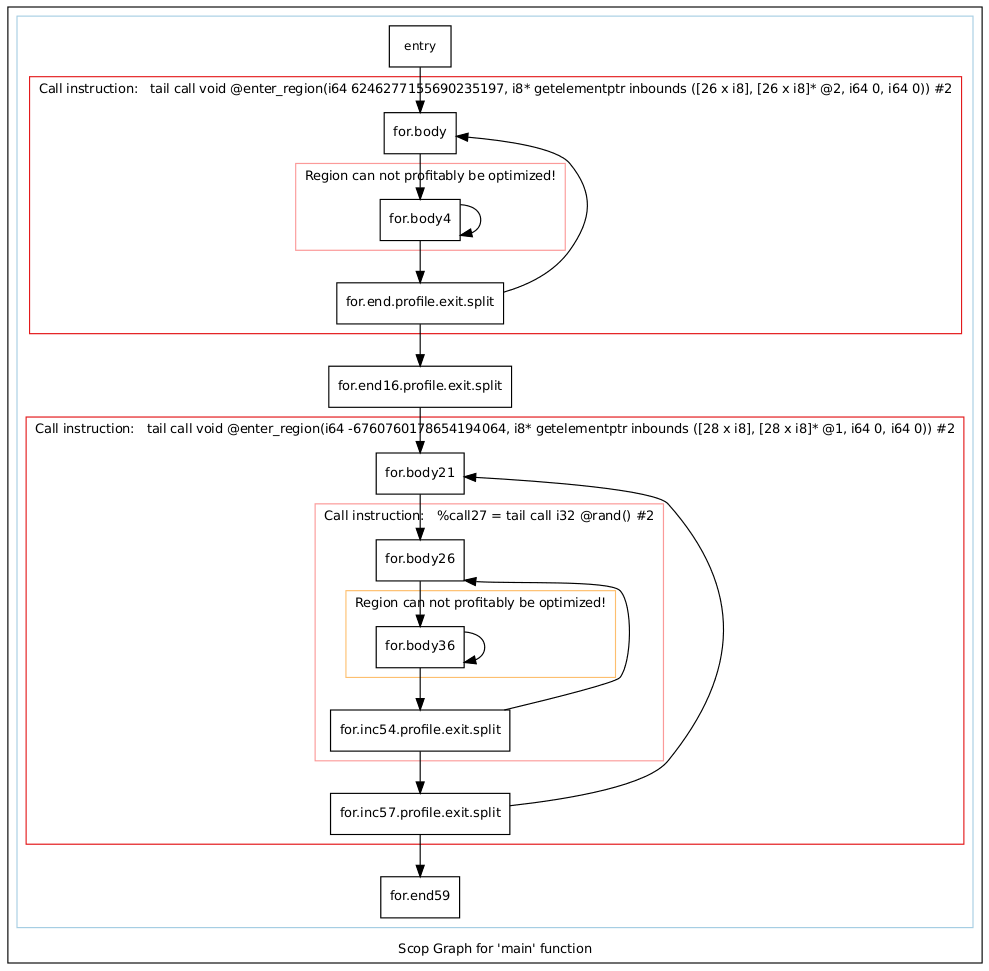
\includegraphics[width=\textwidth]{gfx/matmulScopsAfterInstrumentation.png}
        \label{fig:afterInstrument}
    \end{figure}
    The exact versions of the used software components are listed in \autoref{tab:usedSoftware}.\\
    All measurements are executed on an Intel Xeon E5-2650 v2 machine (2 Sockets with each 8 physical cores each 2.6GHz) with 128GB RAM.
    The precise specifications are listed in \autoref{tab:lscpu} and \autoref{tab:meminfo}.
\end{sloppypar}
\begin{table}[!h]
    \myfloatalign
    \begin{tabularx}{.5\textwidth}{Xc}
        \tableheadline{Name} & \tableheadline{Version}\\ \toprule
        benchbuild           & (2bd0060)\\
        LLVM                 & (04facbb8)\\
        clang                & (89be37b)\\
        polly                & (0fd4fea)\\
        polli                & (697351d)\\
        \bottomrule
    \end{tabularx}
    \caption[Software used for measurements]{
        This table lists the software used for the measurements.
        The components LLVM, clang, polly and polli belong to the compiler infrastructure \llvm itself.
        benchbuild is a program for applying a certain \enquote{experiment} (see \autoref{sec:experimentSettings}) on a selection of programs, distributing them on a SLURM \cite{slurm} cluster and run them.
        (Versions in parenthesis represent short git hashes)
    }
    \label{tab:usedSoftware}
\end{table}

\section{Deviations}\label{sec:deviations}
Only about \usefulRatio of the measured execution times can be used due to on the one hand bugs in the implementation and one the other hand the projects measured which could not be fixed because of time constraints.
The bug in the implementation is occurring in certain constellations of the basic blocks when instrumenting a parent like the following one which is found in the project bzip2 within the file bzlib.c:
\begin{code}
    \caption[Example of a non working parent]{
        This lists a method within the file bzlib.c of the project bzip2.
        The current instrumentation is not working when instrumenting regions within this method.
    }
    \inputminted{c}{c/notWorkingParent.c}
    \label{lst:notWorkingParent}
\end{code}
To cope with it measurements of regions which have a bigger duration than the hole execution time of the project are excluded.
Also measurements of coverages are excluded where the coverage is greater than 100\%.
These occur because the filtering of the obviously bad measurements is not enough to exclude all bad ones.\\
Furthermore for minimizing the influences of the underlying OS multithreading is deactivated, the cluster node is used exclusively, the number of tasks is limited to one and the number of CPUs used per task is limited to 10.
